\documentclass[12pt,letterpaper]{article}
\usepackage{fullpage}
\usepackage[top=2cm, bottom=4.5cm, left=2.5cm, right=2.5cm]{geometry}
\usepackage{amsmath,amsthm,amsfonts,amssymb,amscd}
% \usepackage{lastpage}
\usepackage{enumerate}
\usepackage{fancyhdr}
% \usepackage{mathrsfs}
\usepackage{xcolor}
\usepackage{graphicx}
\usepackage{listings}
\usepackage{hyperref}

\usepackage{float}

% define vector
\newcommand{\q}{\underline}
\newcommand{\mt}{\mathrm}

\setlength{\parindent}{0.2in}
\setlength{\parskip}{0.1in}

% Edit these as appropriate
\newcommand\course{Phys 213}
\newcommand\hwnumber{4}                  % <-- homework number
\newcommand\Name{M.-F. Ho}

\pagestyle{fancyplain}
\headheight 35pt
\lhead{\Name}
\chead{\textbf{\Large Homework 4}}
\rhead{\course \\ \today}
\lfoot{}
\cfoot{}
\rfoot{\small\thepage}
\headsep 1.5em

\newcommand{\Data}{\mathcal{D}}
\newcommand{\xvec}{\boldsymbol{x}}
\newcommand{\Xvec}{\boldsymbol{X}}
\newcommand{\Var}{\textrm{Var}}
\newcommand{\normal}{\textrm{N}}
\newcommand{\uniform}{\textrm{U}}
\newcommand{\xmean}{\langle \xvec \rangle}
\newcommand{\newx}{\tilde{x}}
\newcommand{\integer}{\mathbb{N}}
\newcommand{\thetarv}{\tilde{\theta}}
\newcommand{\phirv}{\tilde{\phi}}

\newcommand{\ml}{m_{\ell}}
\newcommand{\specterms}{^{2S+1}\mathcal{L}^p_\mathcal{J}}
\newcommand{\EWrest}{W^{\mt rest}_\lambda}
\newcommand{\lambdarest}{\lambda_{\textrm{rest}}}

\newcommand{\FeII}{\textrm{Fe\,II}}
\newcommand{\CII}{\textrm{C\,II}}
\newcommand{\columndensity}{N_\ell}
\newcommand{\columndensityrv}{\tilde{\columndensity}}
\newcommand{\kms}{\textrm{\,km/s}}
\newcommand{\dvfwhm}{(\Delta v)_{\textrm{FWHM}}}

\begin{document}

\section*{1 (a): C.O.G}

The approximated equation listed in Draine is:
\begin{equation}
    W \simeq \sqrt{\pi} \frac{b}{c} 
    \frac{\tau_0 }{1 + \tau_0 / (2\sqrt{2})},
\end{equation}
for $\tau_0 < 1.25393$.
And:
\begin{equation}
    W \simeq
    \sqrt{ 
        (\frac{2b}{c})^2 \ln{\frac{\tau_0}{\ln{2}}} +
        \frac{b}{c} \frac{\gamma_{\ell e}\lambda_{\ell u}}{c}
        \frac{(\tau_0 - 1.25393)}{\sqrt{2}}
     },
\end{equation}
for $\tau_0 > 1.25393$.

The question nastily only gives us $W^{\mt rest}_\lambda$ with a unit,
so we have to convert it to the dimensionless $W$.
The conversion should be given in eq (9.4) in Draine:
\begin{equation*}
    W_\lambda = \int d\lambda (1 - e^{-\tau_\nu}) \simeq \lambda_0 W,
\end{equation*}
so ideally we have $W \simeq W_\lambda / \lambda_0$.

\begin{itemize}
    \item Fe II: $W \simeq \EWrest / \lambdarest = 0.051 / 2382.7642 = 2.140 \times 10^{-5}$
    \item Fe II: $W \simeq \EWrest / \lambdarest =  0.0047 / 2249.8768 = 2.089 \times 10^{-6}$
    \item C II:  $W \simeq \EWrest / \lambdarest =  0.060 / 1334.5323 = 4.496 \times 10^{-5}$
\end{itemize}

Now the strategy is to determine which equation to use.
Since we consider ranges $\log{N_{\FeII}} \sim \uniform(12, 16)$ and $\log{N_{\CII}} \sim \uniform(13, 17)$.
Consider the definition of $\tau_0$ as function of $N_\ell$:
\begin{equation}
    \begin{split}
        \tau_{0, \columndensityrv}(\columndensity)
        &= \sqrt{\pi}\frac{e^2}{m_e c} \columndensity
        f_{\ell u} \lambda_{\ell u} \frac{1}{b}(1 - \frac{N_u / g_u}{N_\ell / g_\ell})\\
        &= 1.497 \times 10^{-2} \frac{\mt{cm}^2}{s} \frac{f_{u \ell}\lambda_{\ell u}}{b} N_\ell,
    \end{split}
    \label{eq:tau_0}
\end{equation}

After plugging the numbers into eq~\ref{eq:tau_0}, unfortunately the values of $\tau_0$ is not falling just one-side of the $\tau_0 = 1.25393$:
\begin{equation*}
    \tau_{0,\columndensityrv}(\columndensity, b=10, f=0.320, \lambdarest=2382.7642)
    = (0.11, 1141.44).
\end{equation*}
We thus have to consider both equations.

We clearly know the form of $\tau_0$, so it's a matter of making decisions for plotting.
The way I implemented is estimating $\tau_0$ first based on given $b$ and $\columndensity$, and using the value of $\tau_0$ to determine which equation we are going to use to compute $W$. 
Finally, convert $W$ to $W_{\lambda}$ using $\lambda_0 W$.

Here are examples of dimensionless W C.O.G:
% plotting C.O.G for W
\begin{figure}[H]
    \centering
    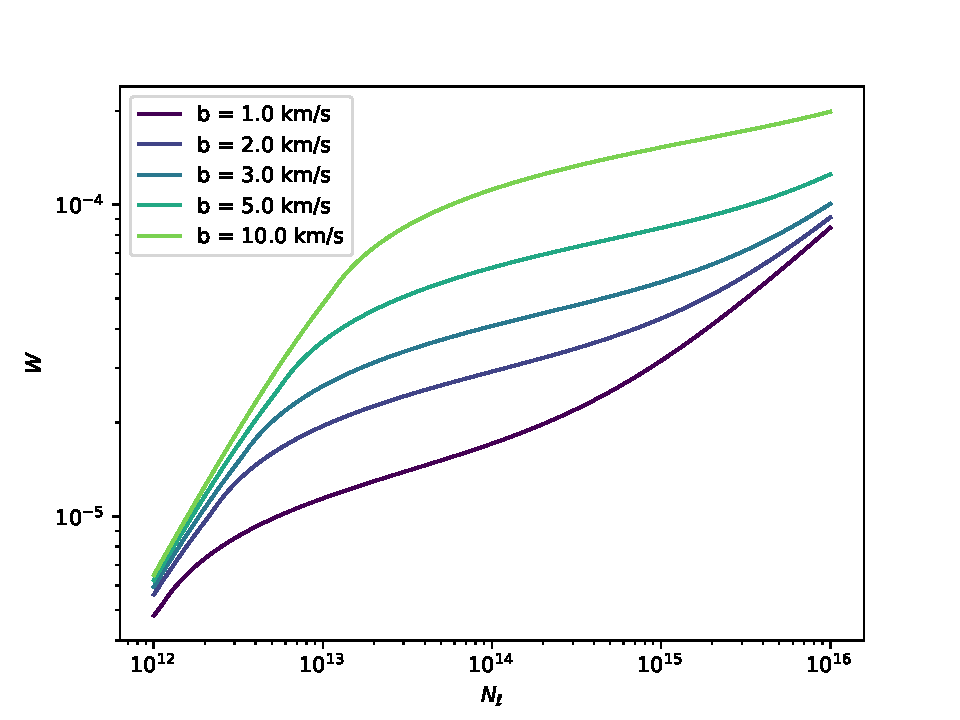
\includegraphics[width=0.75\columnwidth]{images/W_N_Fe_II_1.pdf}
    \caption{Fe II, $\lambdarest = 2382.7642$ \AA}
\end{figure}
\begin{figure}[H]
    \centering
    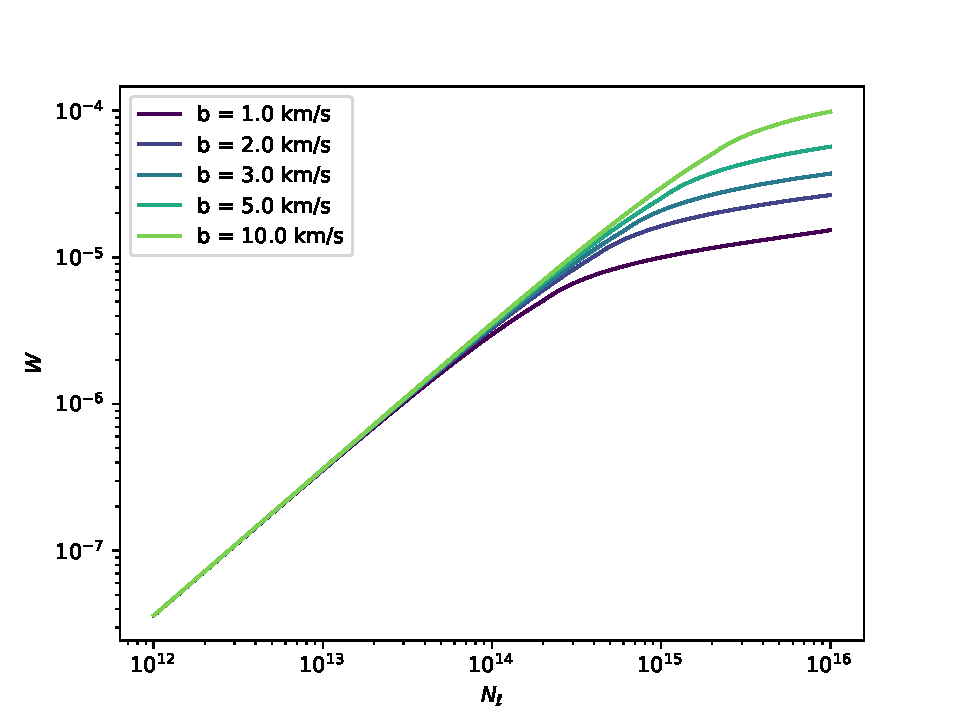
\includegraphics[width=0.75\columnwidth]{images/W_N_Fe_II_2.pdf}
    \caption{Fe II, $\lambdarest = 2249.8768$ \AA}
\end{figure}
\begin{figure}[H]
    \centering
    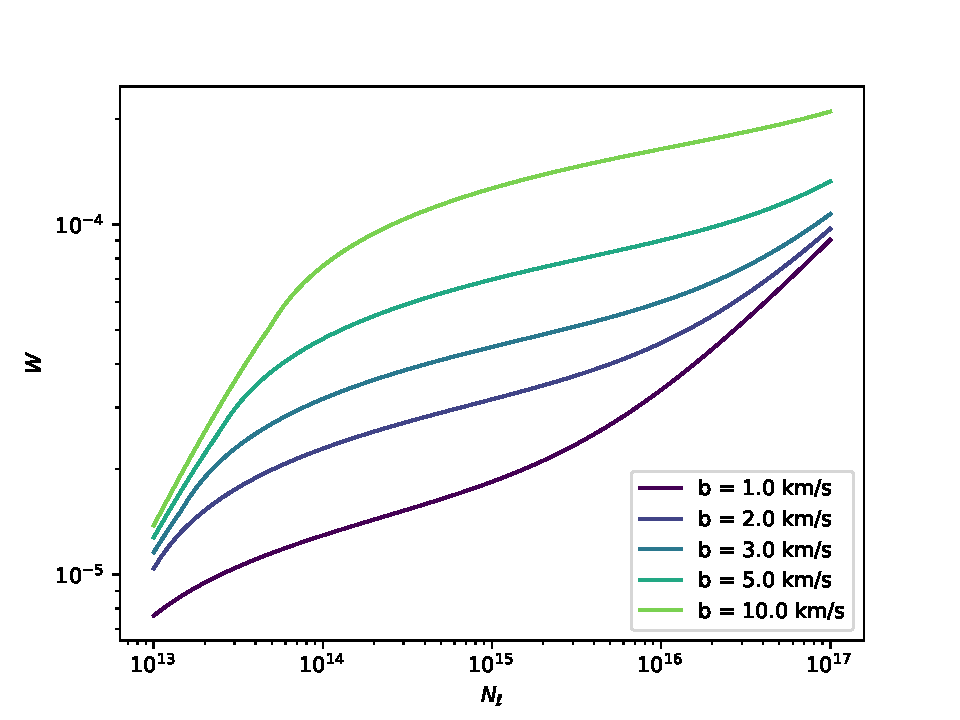
\includegraphics[width=0.75\columnwidth]{images/W_N_C_II.pdf}
    \caption{C II, $\lambdarest = 1134.5323$ \AA}
\end{figure}

Here are examples of $\EWrest$ C.O.G:
% plotting C.O.G for W
\begin{figure}[H]
    \centering
    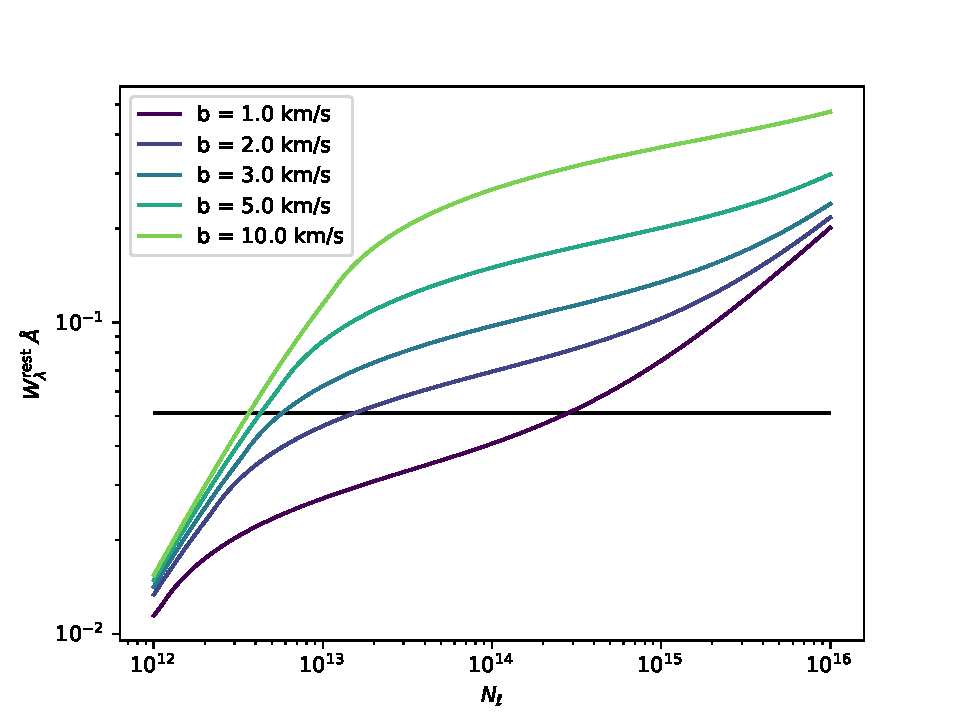
\includegraphics[width=0.75\columnwidth]{images/Wl_N_Fe_II_1.pdf}
    \caption{Fe II, $\lambdarest = 2382.7642$ \AA}
\end{figure}
\begin{figure}[H]
    \centering
    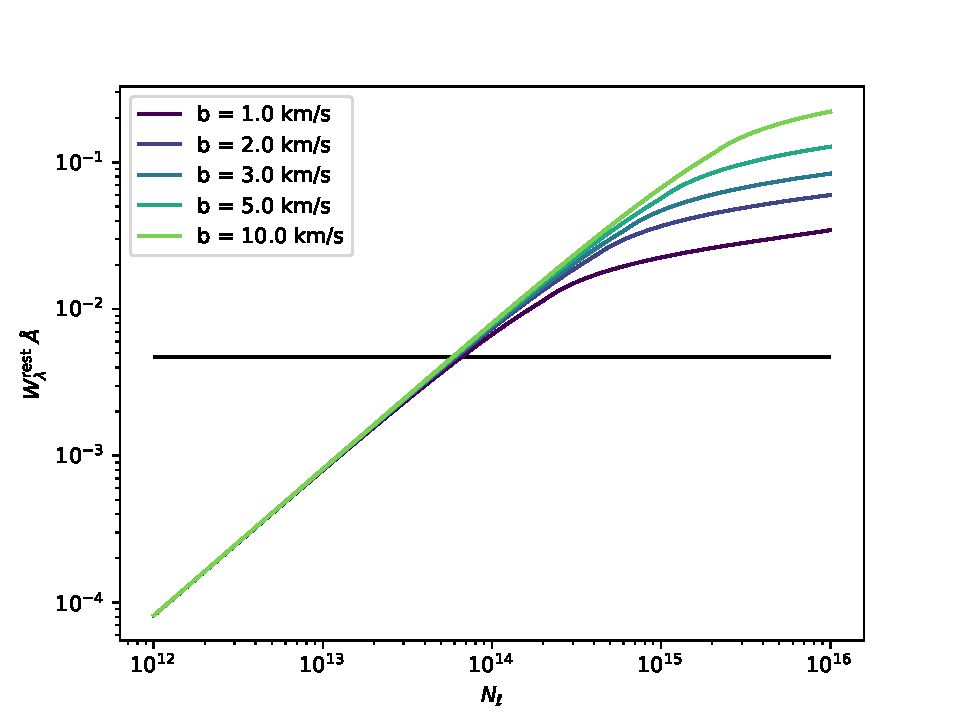
\includegraphics[width=0.75\columnwidth]{images/Wl_N_Fe_II_2.pdf}
    \caption{Fe II, $\lambdarest = 2249.8768$ \AA}
\end{figure}
\begin{figure}[H]
    \centering
    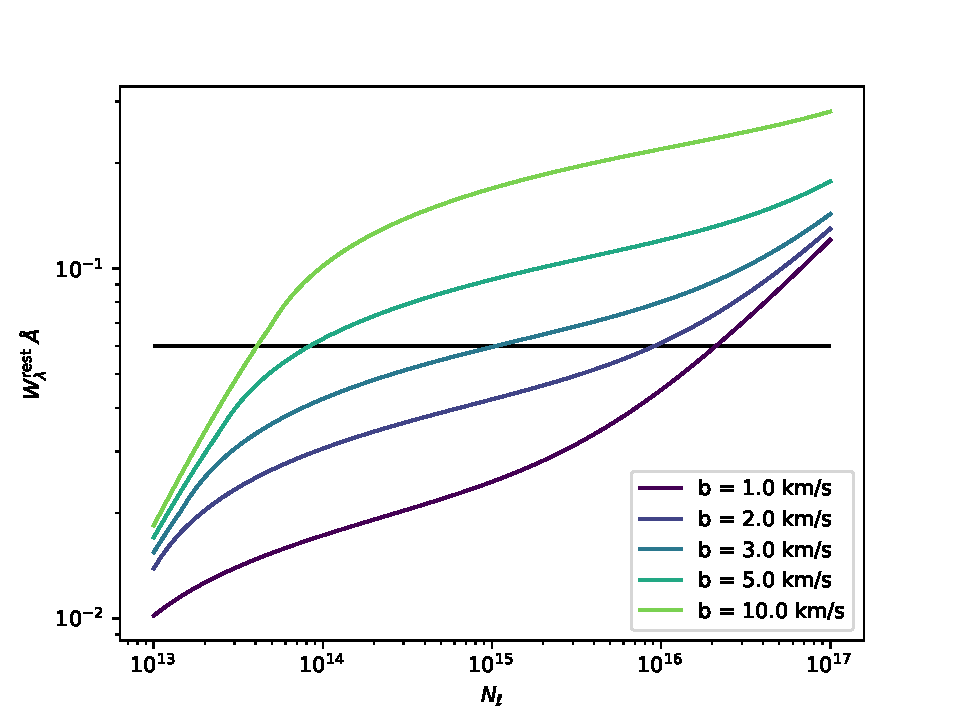
\includegraphics[width=0.75\columnwidth]{images/Wl_N_C_II.pdf}
    \caption{C II, $\lambdarest = 1134.5323$ \AA}
\end{figure}

The black lines I plotted there are the observed $\EWrest$ of these lines.

\section*{1 (b): Fe II Metallicity}
The question asks us to identify the value of b parameters based on the plots we plotted in the question (a).
We probably could solve it analytically, but I think the question asked us to find the value by eyes.

Based on the information given by the question, we have beliefs that $b \in \{ 1, 2, 3, 5, 10\}$ and the column density $\log\columndensity \sim \uniform(12, 16)$.
The trick I think is that our belief only fits to $(b=10\kms, \log{N_\ell} = 16)$ this case.
I am not saying the values are $(b=10\kms, \log{N_\ell} = 16)$, but I am saying if we completely believe our beliefs then the values should like that.

The other Fe II line (the one with $\lambdarest = 2249.8768$ \AA) should have the same $\columndensity = 10^{16}$.
After all they are from the same element.
We thus, by the method of fitting by our eyes, find that $b \simeq 1 \kms $ for the other Fe II line.

Now it's the matter of converting $b$ to $\dvfwhm$.
With the help from Draine:
\begin{equation}
    \dvfwhm = 2 \sqrt{\ln{2}}\, b.
\end{equation}
You can think this is the property of a normal distribution, that the FWHM has a nice relation with the standard deviation.
For these two lines, the first ($\lambdarest = 2382.7642$ \AA):
\begin{equation*}
    \dvfwhm = 2 \sqrt{\ln 2} \, 10 \kms \simeq 17\kms,
\end{equation*}
And for the second ($\lambdarest = 2249.8768$ \AA):
\begin{equation*}
    \dvfwhm = 2 \sqrt{\ln 2} \, 10 \kms \simeq 1.7\kms.    
\end{equation*}

The thing is we should expect the velocity being stretched by the redshifting of the universe by a factor of $(1 + z)$:
\begin{equation}
    \begin{split}
        \dvfwhm^{obs}  &= (1+z) \times 17 \simeq 50 \kms\\
        \dvfwhm^{obs}  &= (1+z) \times 1.7 \simeq 5 \kms.
    \end{split}
\end{equation}

The thing is the resolution of HIRES is around $7-9 \kms$.
Thus, HIRES can resolve the first FeII line but not the second one.

We now are supposed to calculate the metallicity:
\begin{equation}
    [Fe/N] = \log{(N_{Fe} / N_H}) - \log{(N_{Fe} / N_H)}_\odot.
\end{equation}
Now we steal the table from  Asplund et al. 2009,
ARAA, 47, 481, which is suggested by the instructor:
\begin{figure}[H]
    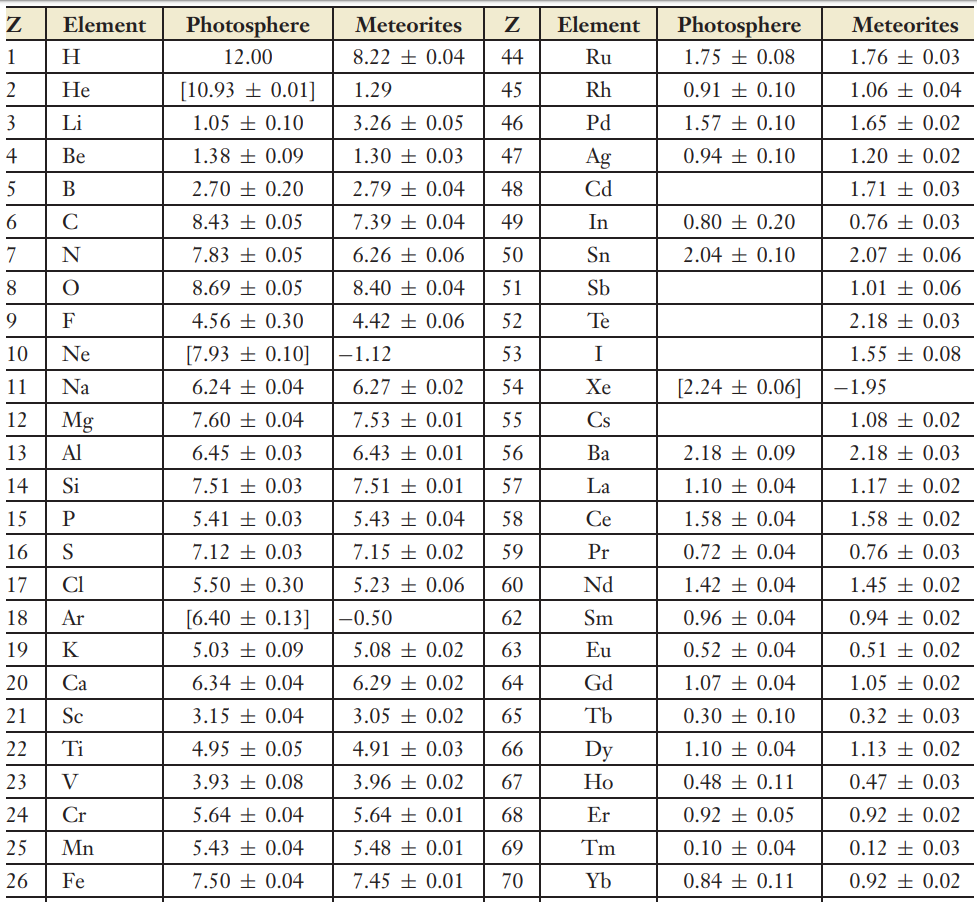
\includegraphics[width=\columnwidth]{images/photosphere.png}
\end{figure}
To compute the solar metallicity, we grab the photosphere values from H and Fe:
\begin{equation*}
    \log{(N_{Fe} / N_H)}_\odot = 7.5 - 12 = -4.5
\end{equation*}
Thus,
\begin{equation*}
    [Fe/H] = 
    \log{(N_{Fe} / N_H)} - \log{(N_{Fe} / N_H)}_\odot =
    \log{(10^{16} / 10^{20.3})} - (-4.5) = 
    16 - 20.3 + 4.5 = 0.2.
\end{equation*}

\section*{1 (c): CII Metallicity}
The question is a little bit obscure for me, since I don't have knowledge about turbulent broadening.
But if we believe the $b$ is broadened by the turbulent, we have high confidence that $b \geq 10 \kms$ but not too far away from $10 \kms$.
And if we highly believe our selection is correct $b \in \{1, 2 ,3, 5, 10\}$ (surely it's not true), 
so combine with two information we have $b \approx 10 \kms$. 
We should note that the only thing we know is $b \geq 10 \kms$ and the turbulent will possibly induce the overestimation of $b$.

We now stop the argument of guessing $b$ and keep going on calculating the metallicity.
Note that based on the plot we find $N_{CII} = 10^{17}$ according to our beliefs on $\log{\columndensity} \sim (13, 17)$.
Now we carry out the metallicity:
\begin{equation*}
    \begin{split}
        [C\,II/H] &= 
        \log{(N_{CII} / N_H)} - \log{(N_{CII} / N_H)}_\odot =\\
        &= \log{(10^{17} / 10^{20.3})} - ( 8.43 - 12 ) \approx 
        17 - 20.3 + 3.57 = 0.27.                
    \end{split}
\end{equation*}
It seems to have a similar metallicity to the Fe\,II metallicity.

\section*{1 (d): Thermally broadening}
We know the thermal velocity is also a Gaussian like distribution, so the FWHM could be written as:
\begin{equation}
    \dvfwhm^{\textrm{thermal}} = 2 \sqrt{\ln 2} \left( \frac{k T}{M} \right)^{1/2} 
    = 2.15 \left( \frac{T / 100\, \mt K}{M / m_H} \right)
    \kms,
\end{equation}
where we know $M_{Fe} / m_H \simeq 56$, and $M_{C} / m_H \simeq 12$.

We would thus be able to infer the value of T if we assume thermal velocity contribute to the $b$ we observe from the plots.

The least condition for these lines being dominated by thermal broadening is that the $\dvfwhm^{\textrm{thermal}} > \dvfwhm^{obs}$.
\begin{equation*}
    \begin{split}
        &\dvfwhm^{\textrm{thermal}} > \dvfwhm^{obs}\\
        &\Rightarrow
        2.15 \left( \frac{T / 100\, \mt K}{M / m_H} \right)
    \kms >  \dvfwhm^{obs}\\
        &\Rightarrow
        T / 100\, {\mt K} > 1/2.15 * \frac{M}{m_H} \dvfwhm^{obs}
    \end{split}
\end{equation*}

Those conditions are:
\begin{itemize}
    \item Fe\,II (2382.7642 \AA): at least 44279\,K
    \item Fe\,II (2249.8768 \AA): at least 4428\,K
    \item C\,II : at least 9488\,K.
\end{itemize}
The temperature for the first one is too high for me to believe.
There're probably something wrong with my beliefs but I am not sure which part went wrong.
For the other two, they are probably going through a plasma stage.

\section*{1(e) Infer b for thermal broadening}
I feel the question is a little bit tricky since it asks us to `infer' the $b$ value and $\columndensity$ instead of asking us to calculate them.
My guess is since it is still in the Doppler broadening region, let's plot more b values:
\begin{figure}[H]
    \centering
    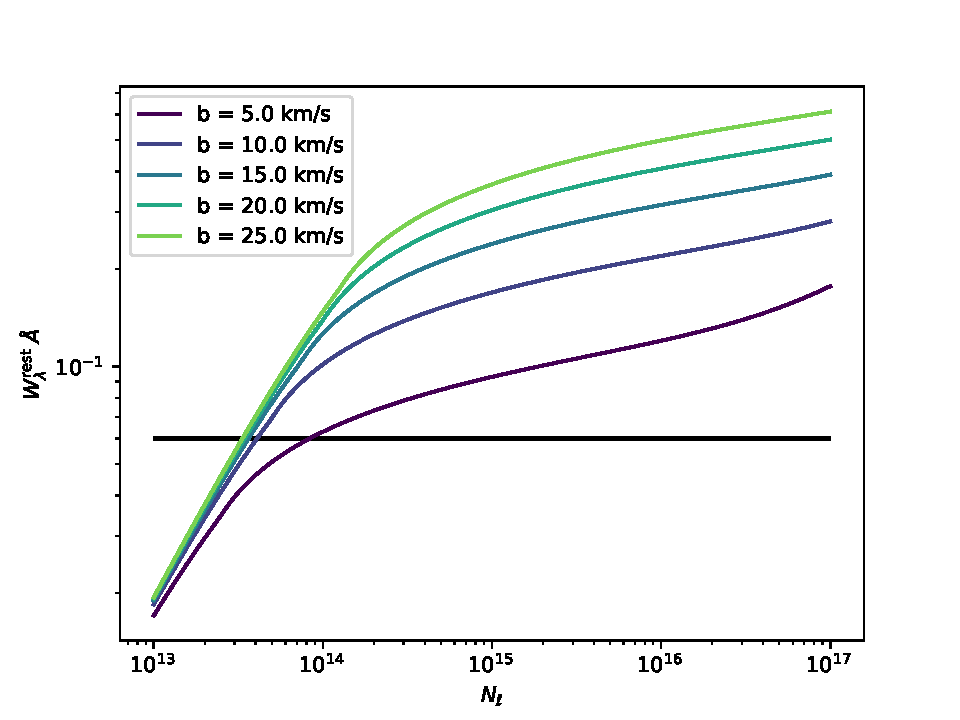
\includegraphics[width=0.75\columnwidth]{images/Wl_N_C_II_more_b.pdf}
\end{figure}
If $b = 25 \kms$, it is still in the Doppler broadening region but the curve reach the measured $\EWrest$ line.

The value of metallicity would be the same since the column density seems to be unchanged:
\begin{equation*}
    \begin{split}
        [C\,II/H] &= 
        \log{(N_{CII} / N_H)} - \log{(N_{CII} / N_H)}_\odot =\\
        &= \log{(10^{17} / 10^{20.3})} - ( 8.43 - 12 ) \approx 
        17 - 20.3 + 3.57 = 0.27.                
    \end{split}
\end{equation*}

I guess the idea is if it is all due to Doppler broadening, then the $\EWrest$ measure should fall into the flat regime of the C.O.G.
\begin{figure}
    \centering
    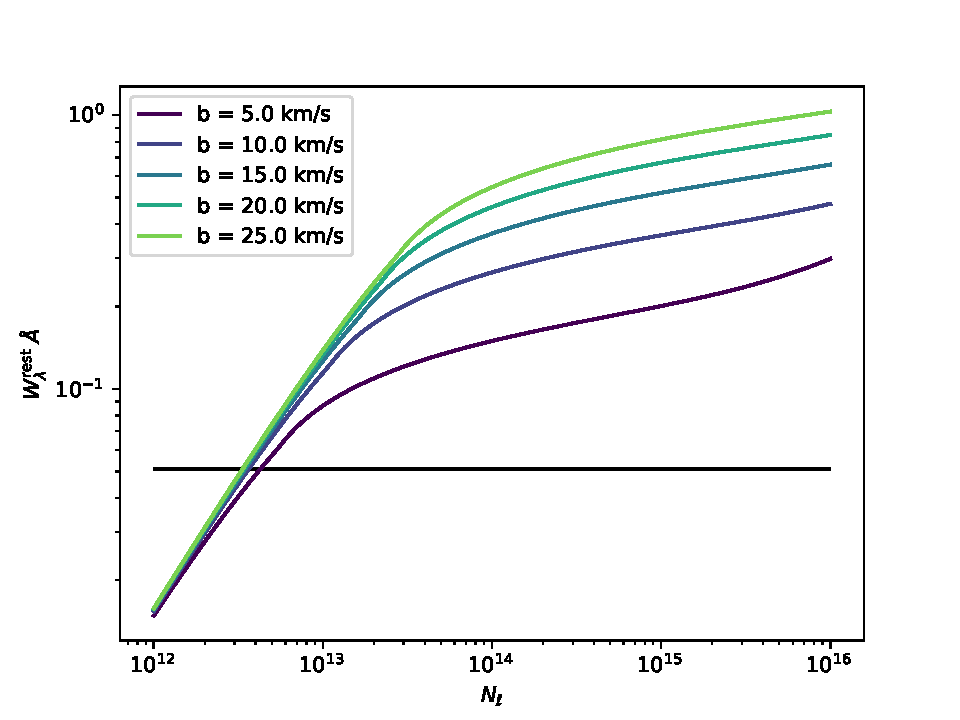
\includegraphics[width=0.75\columnwidth]{images/Wl_N_Fe_II_1_more_b.pdf}
\end{figure}
So if $b = 25 \kms$, we probably have a lower $\columndensity$ in Fe.
So the abundance of carbon comparing to Fe will increase.

\section*{1 (f): Carbon enhanced}
Given that carbon rich DLA is rare, it's probably not possible that the lines are due to Doppler broadening.
The way to decrease the column density of carbon is to increase the $b$, in that way it is in the optically thin regime.
Usually it is hard to resolve the lines in optically thin regime though we have a relatively larger $b$ here for carbon.
But if we know the combination of the elements in the medium, we could try to use other lines in Doppler or damping regimes so that would be easier to resolve.

\end{document}
